\documentclass[8pt,dvipsnames]{beamer}
\usepackage[T1]{fontenc}
\usepackage{libertinus}
\usepackage{amsmath}
\usepackage[most]{tcolorbox}
\usepackage{graphicx}

\usepackage{hyperref}
%python 
\usepackage{listings}
% Default fixed font does not support bold face
\DeclareFixedFont{\ttb}{T1}{txtt}{bx}{n}{8} % for bold
\DeclareFixedFont{\ttm}{T1}{txtt}{m}{n}{8}  % for normal

% Custom colors
\usepackage{color}
\definecolor{deepblue}{rgb}{0,0,0.5}
\definecolor{deepred}{rgb}{0.6,0,0}
\definecolor{deepgreen}{rgb}{0,0.5,0}

\usepackage{listings}

% Python style for highlighting
\newcommand\pythonstyle{\lstset{
		language=Python,
		basicstyle=\ttm,
		morekeywords={self},              % Add keywords here
		keywordstyle=\ttb\color{deepblue},
		emph={MyClass,__init__},          % Custom highlighting
		emphstyle=\ttb\color{deepred},    % Custom highlighting style
		stringstyle=\color{deepgreen},
		frame=tb,                         % Any extra options here
		showstringspaces=false
}}


% Python environment
\lstnewenvironment{python}[1][]
{
	\pythonstyle
	\lstset{#1}
}
{}

% Python for external files
\newcommand\pythonexternal[2][]{{
		\pythonstyle
		\lstinputlisting[#1]{#2}}}

% Python for inline
\newcommand\pythoninline[1]{{\pythonstyle\lstinline!#1!}}

\usepackage{xcolor}  
\newcommand{\cb}[1]{{\color{CadetBlue}#1}}

\usepackage{pgfplots}
\pgfplotsset{compat=newest}
\setlength{\parskip}{0.5em}

\usepackage{setspace}
\setstretch{1.25}  
\usetheme{Singapore}
\setbeamertemplate{navigation symbols}{}


\title{CSE574 Introduction to Machine Learning}
\subtitle{Advance Practices and Unsupervised Learning: k-nearest neighbors}
\author{Jue Guo}
\institute{University at Buffalo}
\date{\today}

\begin{document}
\begin{frame}
	\titlepage
\end{frame}
\begin{frame}
	\frametitle{Outline}
	\tableofcontents
\end{frame}
\section{k-nearest neighbors}
\begin{frame}{k-nearest neighbors}
	\textbf{Learning Objective}
	\begin{itemize}
		\item Define k-nearest neighbors.
		\item List the steps of the k-nearest neighbors algorithm.
		\item Explain how to choose an appropriate value of \(k\).
		\item Use a decision boundary plot to explore different values of \(k\).
		\item Define Euclidean distance, Minkowski distance, and Manhattan distance.
		\item Implement k-nearest neighbors using scikit-learn.
	\end{itemize}
	We will do a signup sheet to track attendance at the end of class today.
\end{frame}

\begin{frame}{k-nearest neighbor}

	\textbf{\(\boldsymbol{k}\)-nearest neighbors} is a supervised classification algorithm that predicts the class of an output feature based on the class of other instances with the most similar, or "nearest," input features.
	\begin{itemize}
		\item  The \(k\) nearest instances, or neighbors, are identified using some distance measure, and the classes of each neighbor's output feature are identified.
	\end{itemize}
	The most frequently occurring class from the \(k\) closest instances becomes the prediction.

	Let's look at an example for k-nearest neighbor;

\end{frame}

\begin{frame}{An Example: Classifying penguins based on bill length:}
	\begin{columns}
		\column{0.5\textwidth}
		\begin{figure}
			\centering
			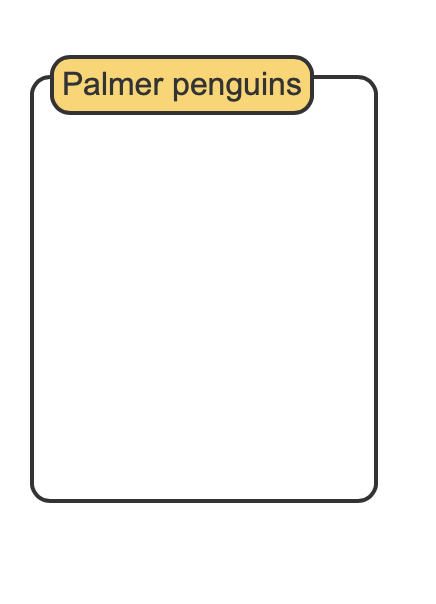
\includegraphics[width=\textwidth]{imgs/knn_1.png}
		\end{figure}
		\column{0.5\textwidth}
		\begin{itemize}
			\item The Palmer penguins dataset was collected by researchers studying penguins on the Palmer Archipelago in Antarctica.
		\end{itemize}
	\end{columns}
\end{frame}

\begin{frame}{}
	\begin{columns}
		\column{0.5\textwidth}
		\begin{figure}
			\centering
			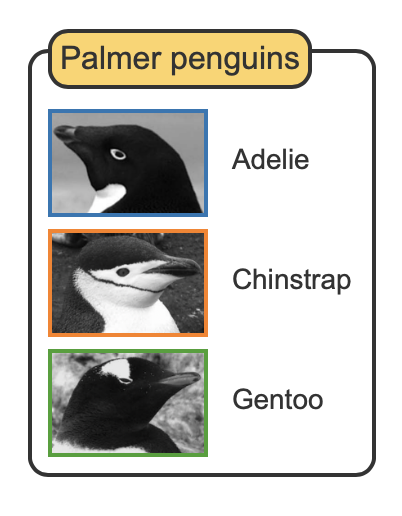
\includegraphics[width=\textwidth]{imgs/knn_2.png}
		\end{figure}
		\column{0.5\textwidth}
		\begin{itemize}
			\item Three species of penguins were studied: Adelie, Chinstrap, and Gentoo.
		\end{itemize}
	\end{columns}
\end{frame}

\begin{frame}{}
	\begin{itemize}
		\item Body measurements were taken from each penguin, including bill length and bill depth.
	\end{itemize}
	\begin{figure}
		\centering
		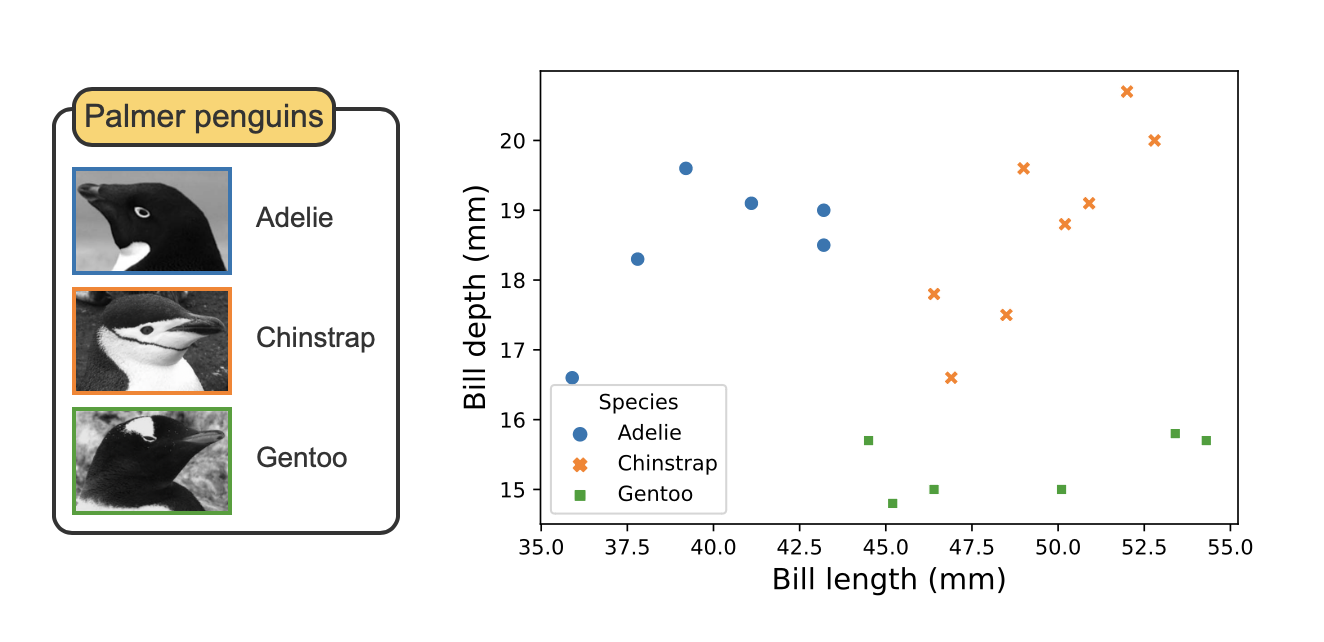
\includegraphics[width=\textwidth]{imgs/knn_3.png}
	\end{figure}
\end{frame}

\begin{frame}
	\begin{itemize}
		\item Suppose an unknown penguin has a bill length of 45 mm and a bill depth of 19 mm. Which species is most likely for this penguin?
	\end{itemize}
	\begin{figure}[ht]
		\centering
		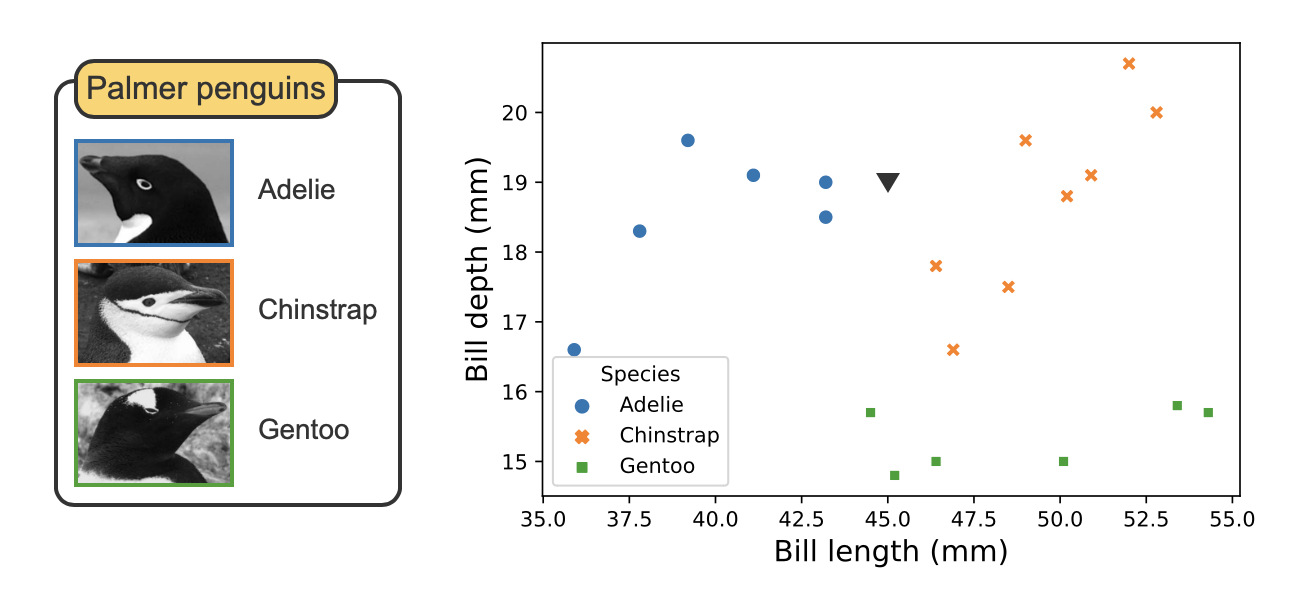
\includegraphics[width=\linewidth]{imgs/knn_4.png}
	\end{figure}
\end{frame}

\begin{frame}
	\begin{itemize}
		\item The three nearest penguins to (45, 19) are identified. Two are Adelie penguins, and one is a Chinstrap penguin.
	\end{itemize}
	\begin{figure}[ht]
		\centering
		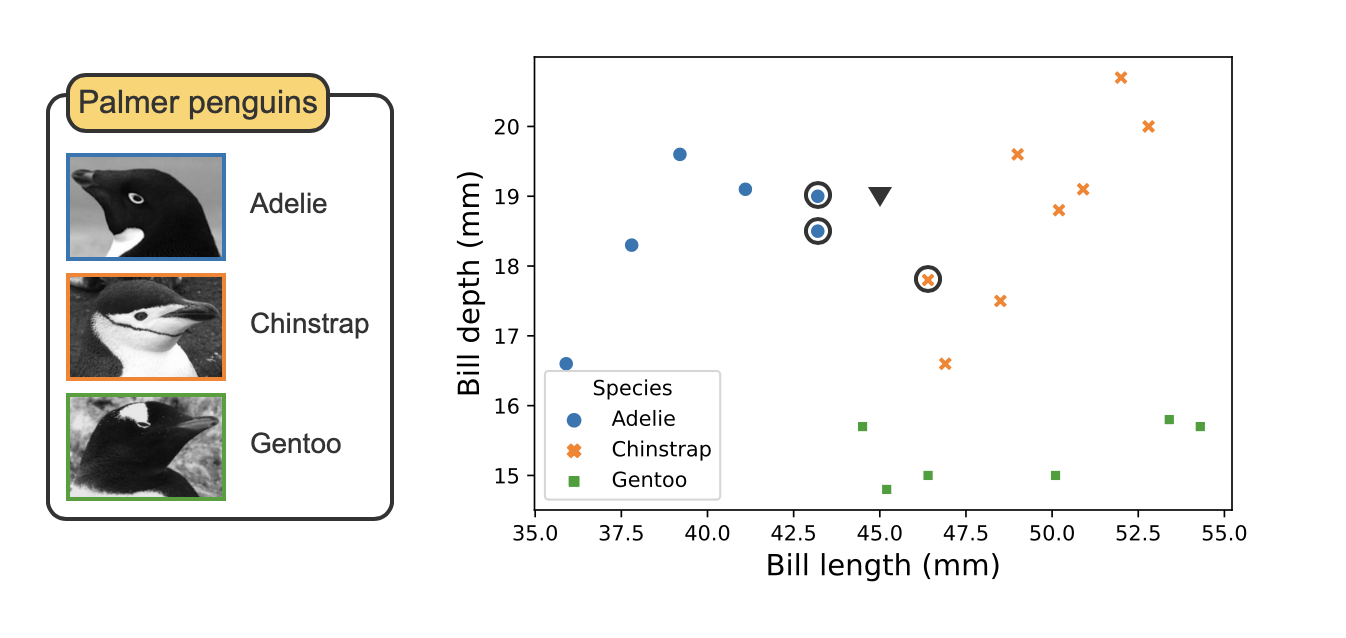
\includegraphics[width=\linewidth]{imgs/knn_5.png}
	\end{figure}
\end{frame}

\begin{frame}
	\begin{itemize}
		\item 2/3 = 67 \% of the nearest penguins are Adelie. So, a penguin at (45, 19) is predicted to be an Adelie penguin.
	\end{itemize}
	\begin{figure}[ht]
		\centering
		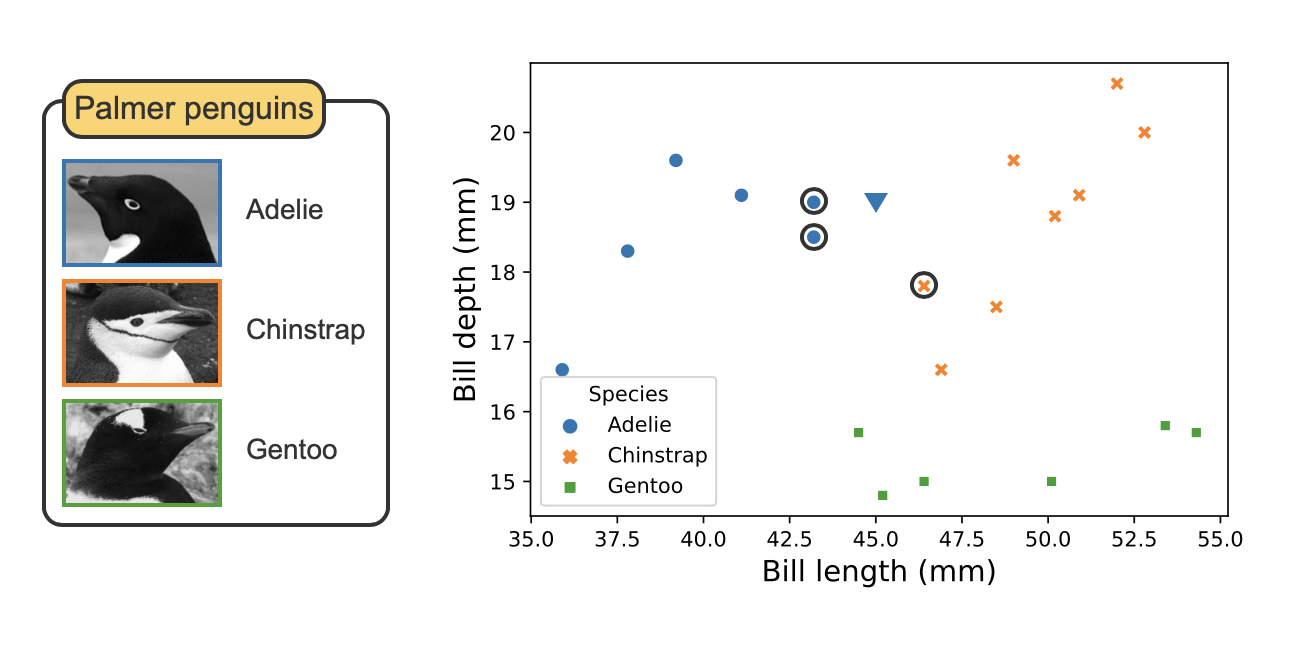
\includegraphics[width=\linewidth]{imgs/knn_6.png}
	\end{figure}
\end{frame}

\begin{frame}{Practice Questions}
	A penguin with unknown species has a bill length of 48 mm and a bill depth of 16 mm (black triangle). The five nearest neighbors for this penguin are circled in the scatter plot below.
	\begin{figure}[ht]
		\centering
		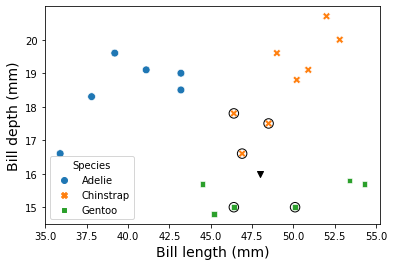
\includegraphics[scale=0.5]{imgs/knn_7.png}
	\end{figure}
\end{frame}

\section{k-nearest neighbors algorithm}
\begin{frame}{k-nearest neighbors algorithm}
	Let \(\mathbf{x}_{i}=\left(x_{1 i}, x_{2 i}, \ldots, x_{p i}\right)\) denote the \(p\) input features from instance \(i\), and let \(y_{i}\) denote the output feature. Let \(n\) denote the number of instances in a dataset. A new instance \(x^{*}\) is classified in k-nearest neighbors by identifying the \(k\)-nearest instances to \(x^{*}\), and assigning the most common class as the prediction.
	\begin{figure}[ht]
		\centering
		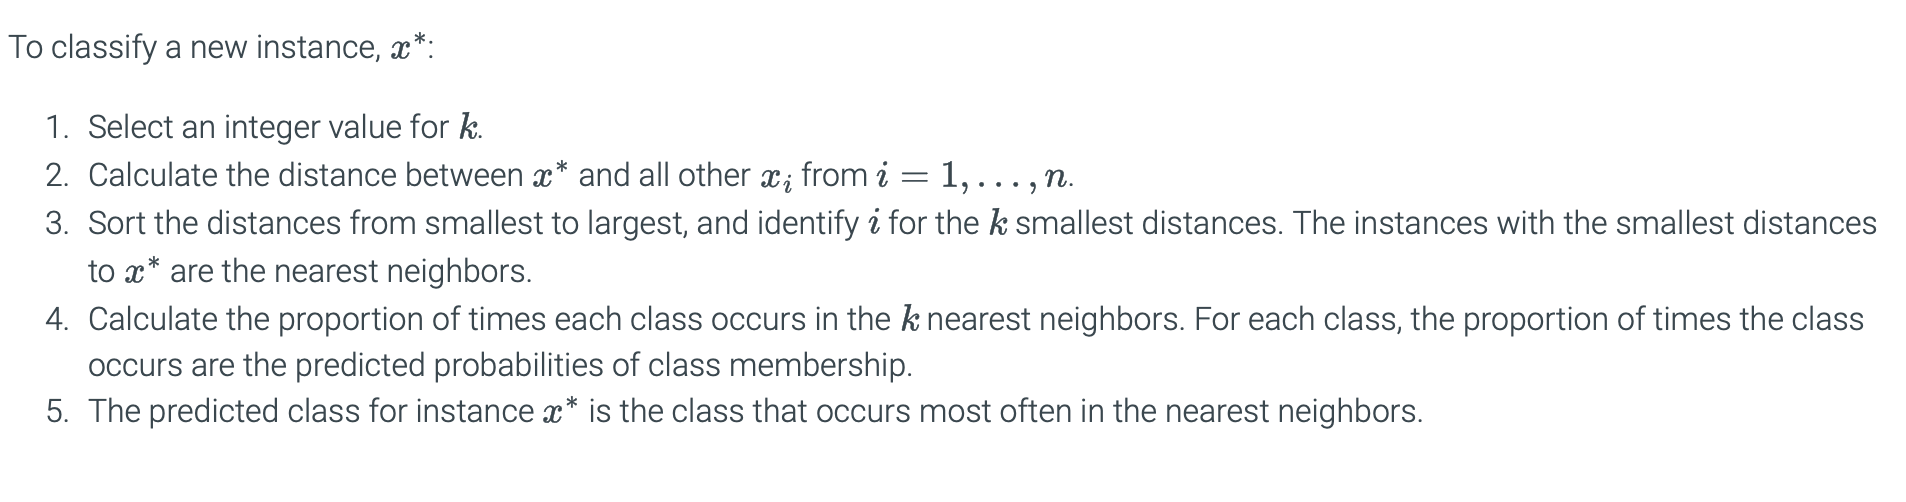
\includegraphics[width=\linewidth]{imgs/knn_8.png}
	\end{figure}
\end{frame}

\begin{frame}{Applying the Algorithm}
	\begin{figure}[ht]
		\centering
		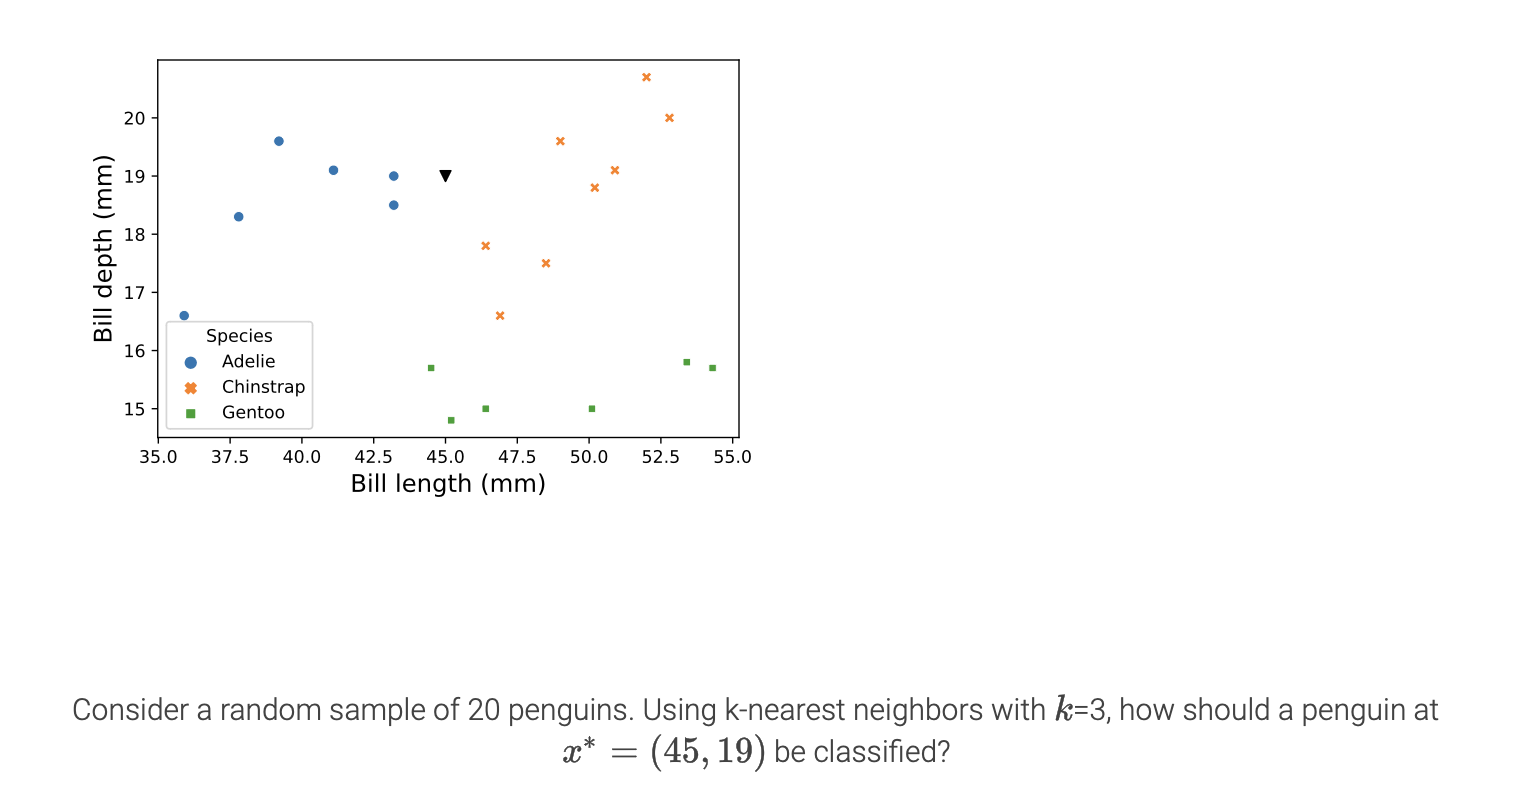
\includegraphics[width=\linewidth]{imgs/knn_9.png}
	\end{figure}
\end{frame}

\begin{frame}
	\begin{figure}[ht]
		\centering
		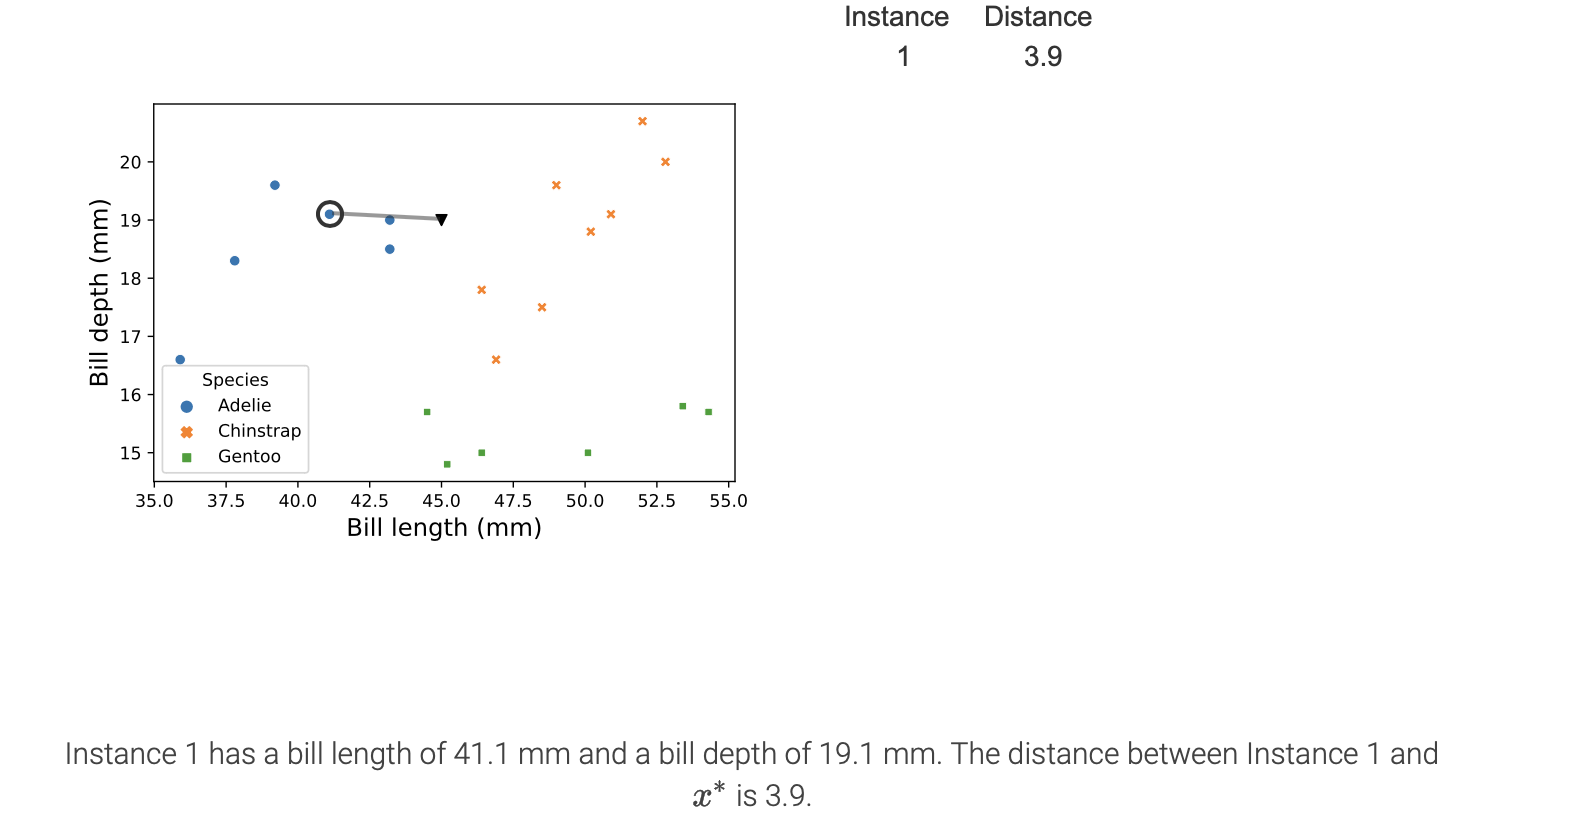
\includegraphics[width=\linewidth]{imgs/knn_10.png}
	\end{figure}
\end{frame}

\begin{frame}
	\begin{figure}[ht]
		\centering
		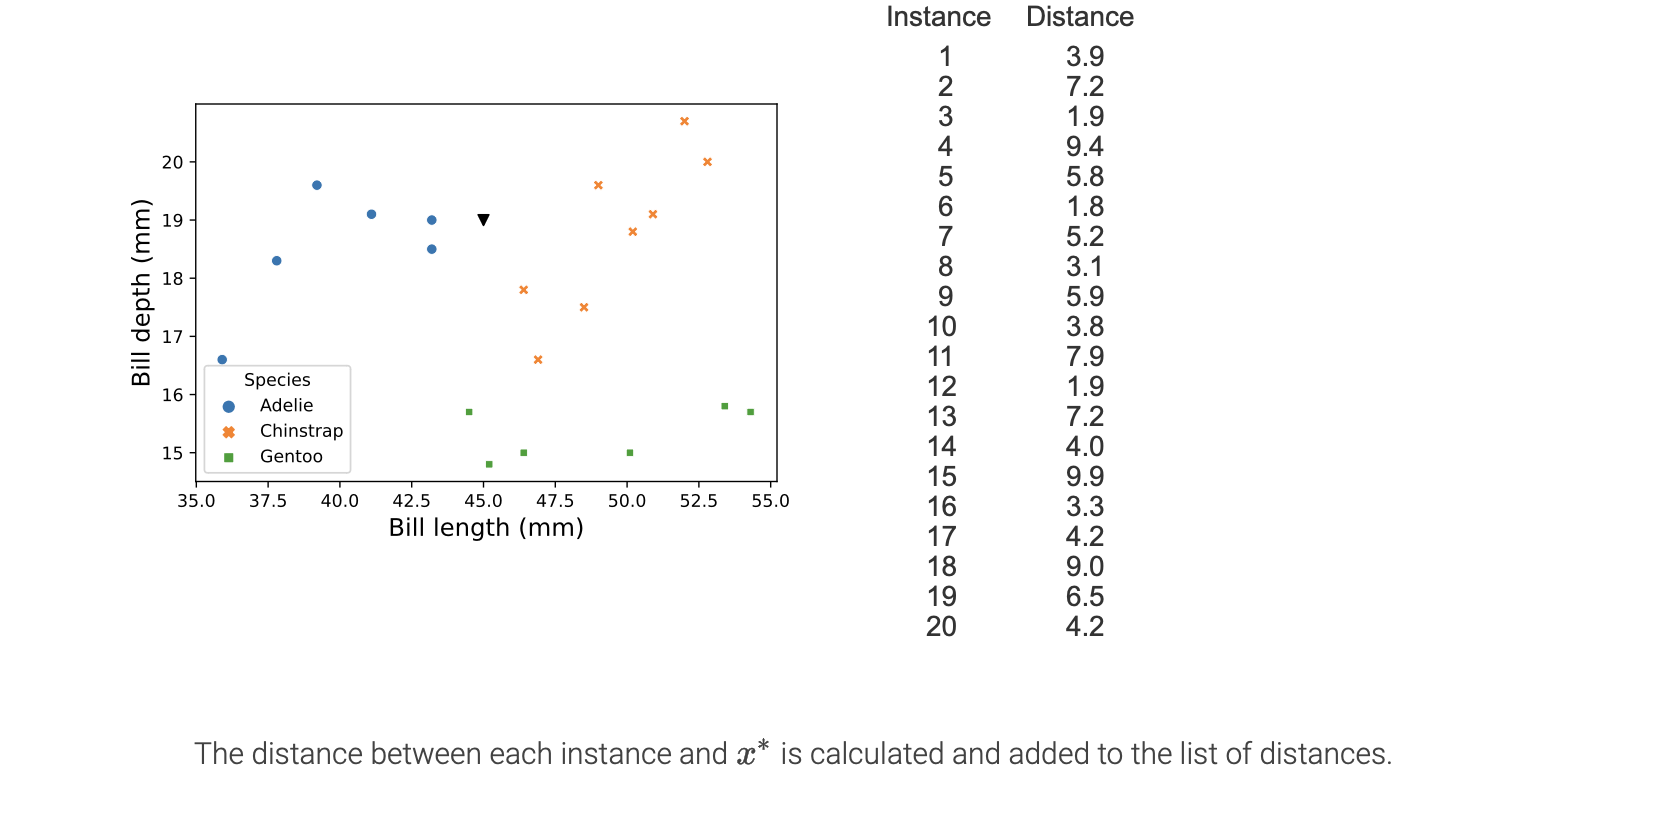
\includegraphics[width=\linewidth]{imgs/knn_11.png}
	\end{figure}
\end{frame}

\begin{frame}
	\begin{figure}[ht]
		\centering
		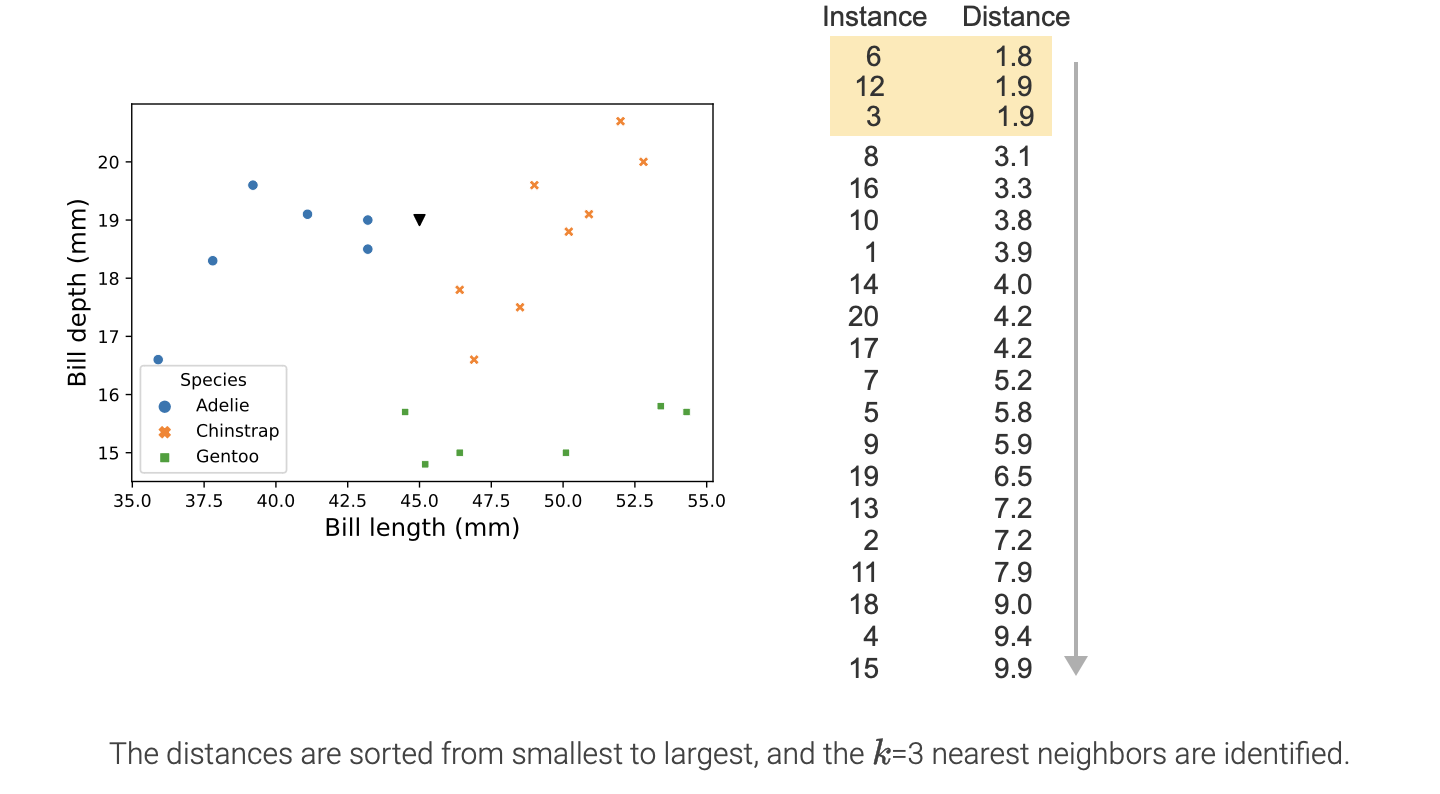
\includegraphics[width=\linewidth]{imgs/knn_12.png}
	\end{figure}
\end{frame}

\begin{frame}
	\begin{figure}[ht]
		\centering
		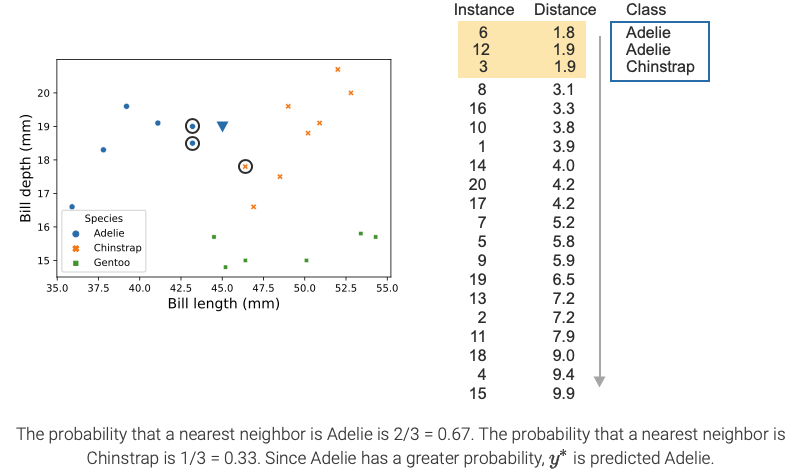
\includegraphics[width=\linewidth]{imgs/knn_13.png}
	\end{figure}
\end{frame}

\begin{frame}{Practice Round: Steps of the k-nearest neighbors algorithm.}
	\begin{figure}[ht]
		\centering
		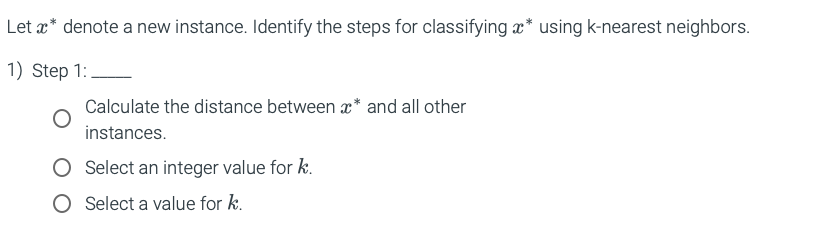
\includegraphics[width=\linewidth]{imgs/knn_14.png}
	\end{figure}
\end{frame}

\begin{frame}
	\begin{figure}[ht]
		\centering
		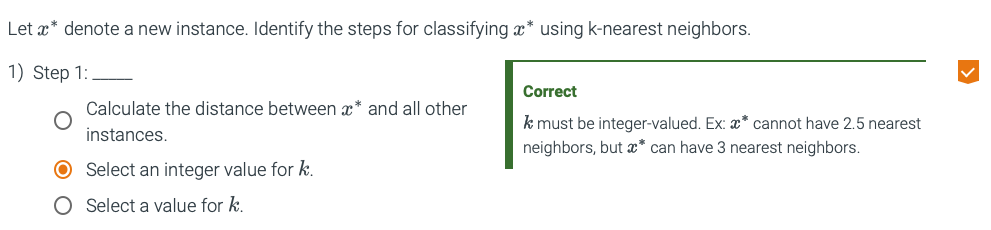
\includegraphics[width=\linewidth]{imgs/knn_15.png}
	\end{figure}
\end{frame}
\begin{frame}
	\begin{figure}[ht]
		\centering
		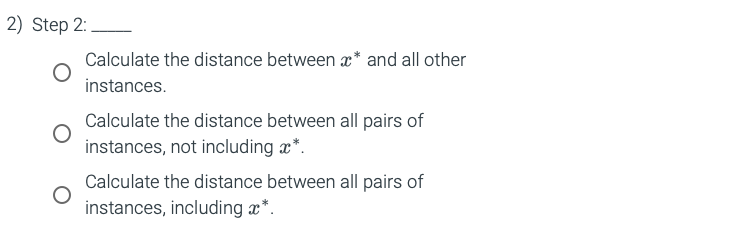
\includegraphics[width=\linewidth]{imgs/knn_16.png}
	\end{figure}
\end{frame}

\begin{frame}
	\begin{figure}[ht]
		\centering
		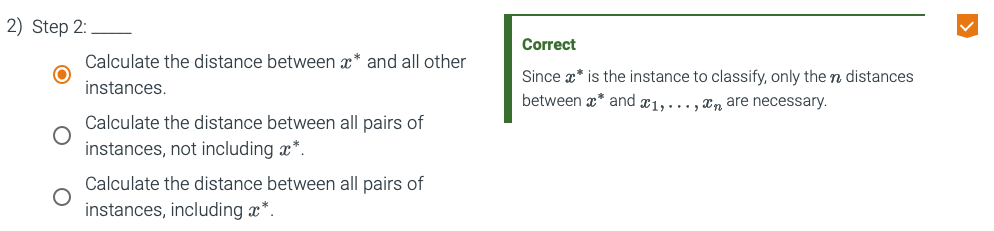
\includegraphics[width=\linewidth]{imgs/knn_17.png}
	\end{figure}
\end{frame}

\begin{frame}
	\begin{figure}[ht]
		\centering
		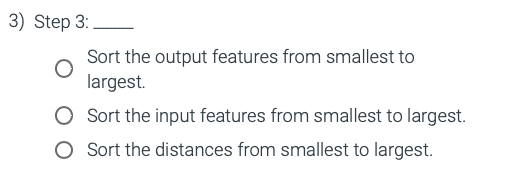
\includegraphics[scale=0.5]{imgs/knn_18.png}
	\end{figure}
\end{frame}

\begin{frame}
	\begin{figure}[ht]
		\centering
		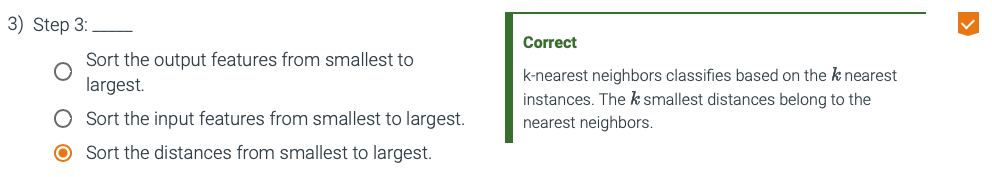
\includegraphics[width=\linewidth]{imgs/knn_19.png}
	\end{figure}
\end{frame}

\begin{frame}
	\begin{figure}[ht]
		\centering
		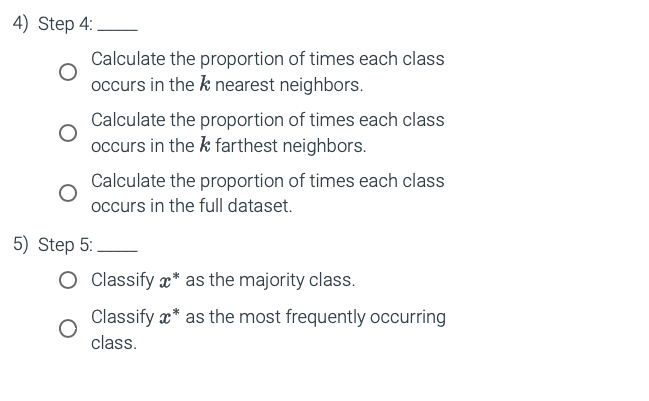
\includegraphics[width=\linewidth]{imgs/knn_20.png}
	\end{figure}
\end{frame}

\begin{frame}
	\begin{figure}[ht]
		\centering
		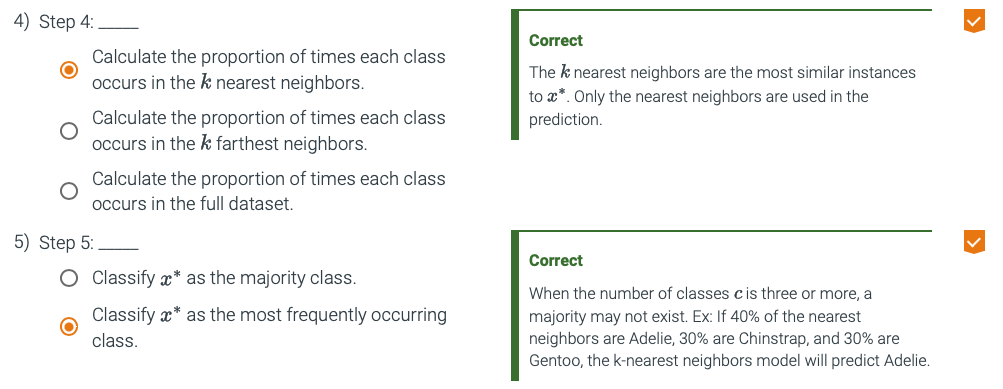
\includegraphics[width=\linewidth]{imgs/knn_21.png}
	\end{figure}
\end{frame}

\section{Selecting an appropriate k}
\begin{frame}{Selecting an appropriate k}
	A \textbf{hyperparameter} is a user-defined setting in a machine learning model that is not estimated during model fitting.
	\begin{itemize}
		\item Changing the values of a hyperparameter affects the model's performance and predictions.
		\item k-nearest neighbors is sensitive to two hyperparameters: the value of \(k\) and the distance measure. Models with different values of \(k\) may result in different predictions.
		\item Setting \(k\) too small results in predictions that are based on only a few instances and thus highly variable.
		\item But setting \(k\) too large often leads to models that are underfit. In practice, \(k\) is usually set between 3 and 15 .
	\end{itemize}
\end{frame}

\begin{frame}
	\begin{figure}[ht]
		\centering
		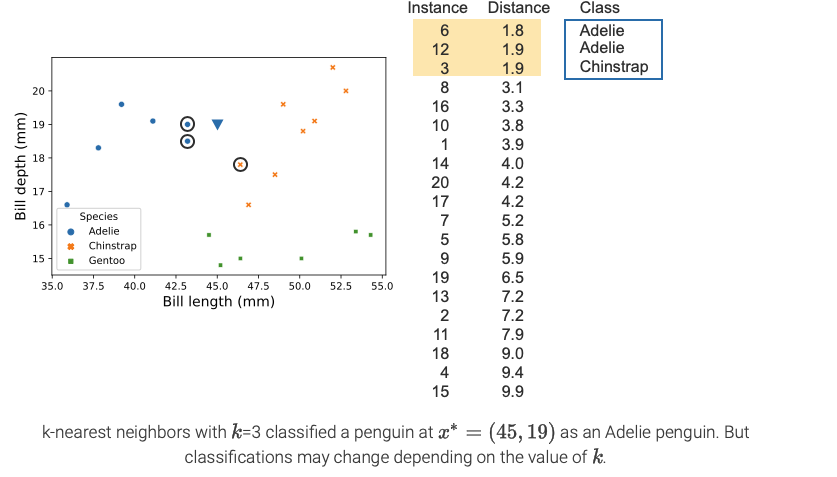
\includegraphics[width=\linewidth]{imgs/knn_22.png}
	\end{figure}
\end{frame}

\begin{frame}
	\begin{figure}[ht]
		\centering
		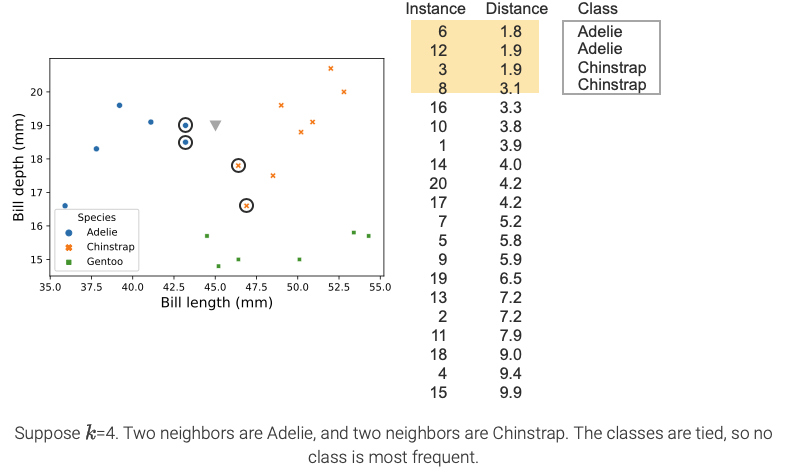
\includegraphics[width=\linewidth]{imgs/knn_23.png}
	\end{figure}
\end{frame}

\begin{frame}
	\begin{figure}[ht]
		\centering
		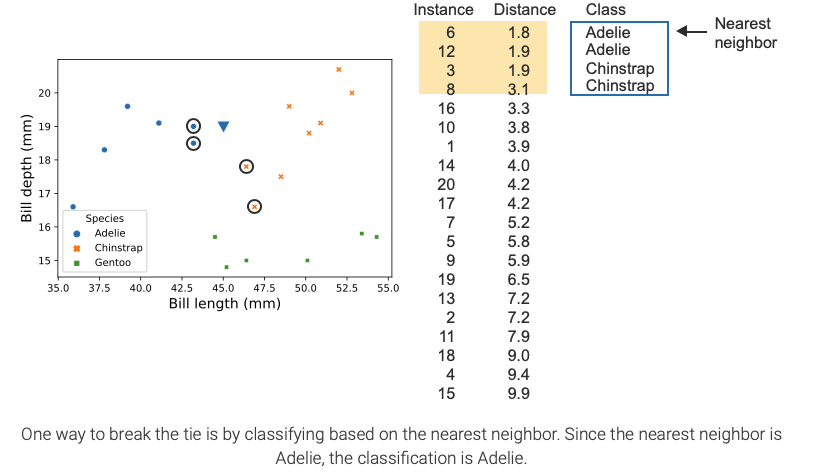
\includegraphics[width=\linewidth]{imgs/knn_24.png}
	\end{figure}
\end{frame}

\begin{frame}
	\begin{figure}[ht]
		\centering
		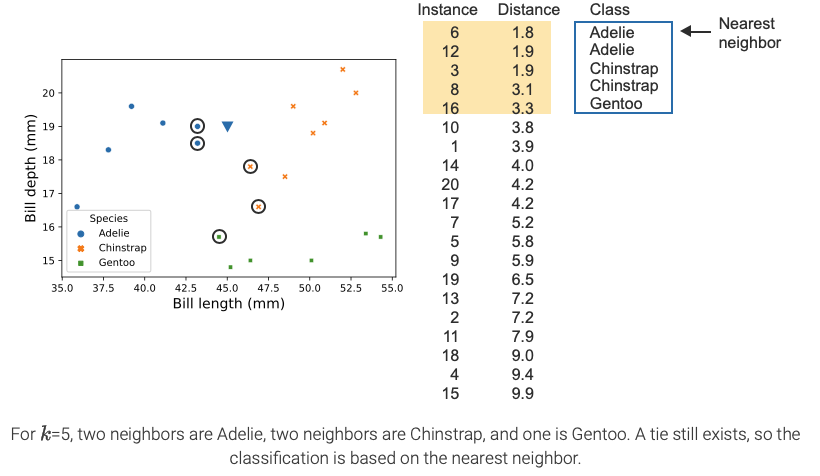
\includegraphics[width=\linewidth]{imgs/knn_25.png}
	\end{figure}
\end{frame}

\begin{frame}
	\begin{figure}[ht]
		\centering
		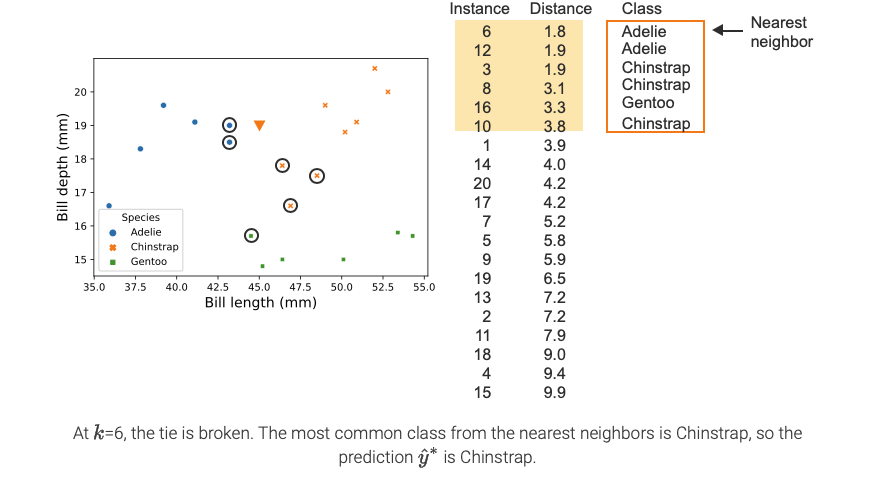
\includegraphics[width=\linewidth]{imgs/knn_26.png}
	\end{figure}
\end{frame}

\begin{frame}
	\begin{figure}[ht]
		\centering
		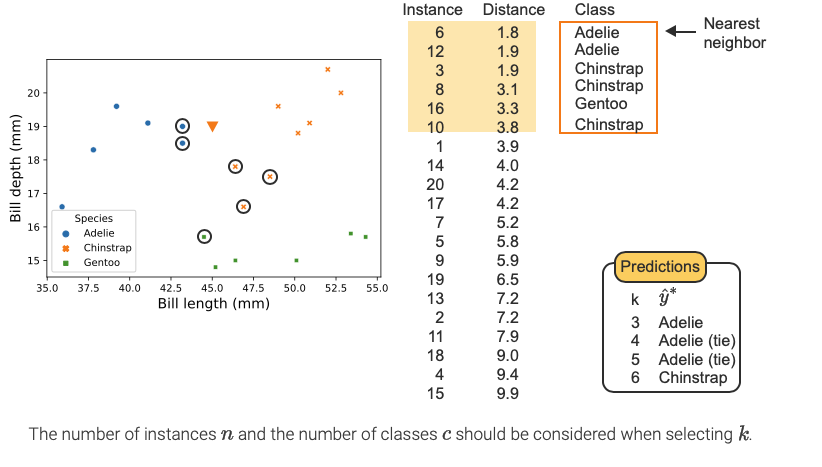
\includegraphics[width=\linewidth]{imgs/knn_27.png}
	\end{figure}
\end{frame}

\begin{frame}{Practice Questions}
	\begin{figure}[ht]
		\centering
		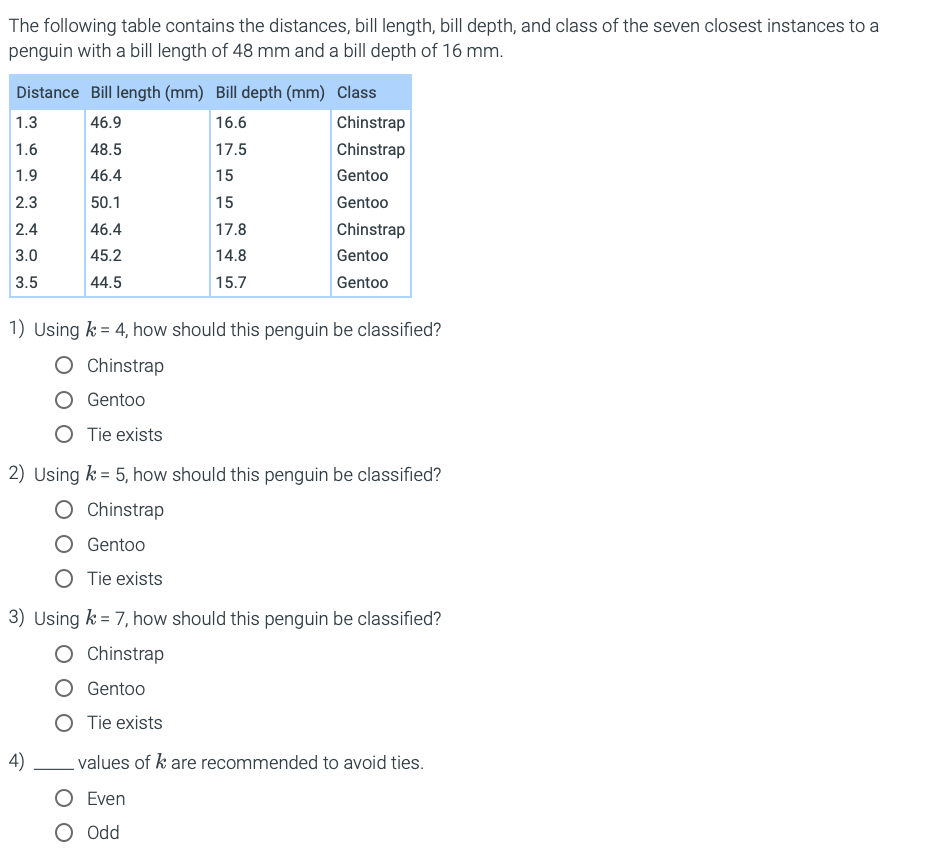
\includegraphics[scale=0.25]{imgs/knn_28.png}
	\end{figure}
\end{frame}

\section{Decision Boundaries}
\begin{frame}
	\frametitle{Decision Boundaries}
	Decision boundaries represent the dividing line between predicting one class vs. another class.
	\begin{itemize}
		\item Decision boundaries may be visualized using a scatter plot for one or two input features, or multiple scatter plots when the number of input features \(p>2\).
		\item Examining a decision boundary plot helps researchers understand the predictions of a machine learning model and
		      identify a model's strengths and weaknesses.
		\item Decision boundary plots are also useful tools for comparing models.
	\end{itemize}
\end{frame}

\begin{frame}
	\frametitle{Exploring classification models with decision boundary plots.}
	\begin{figure}[ht]
		\centering
		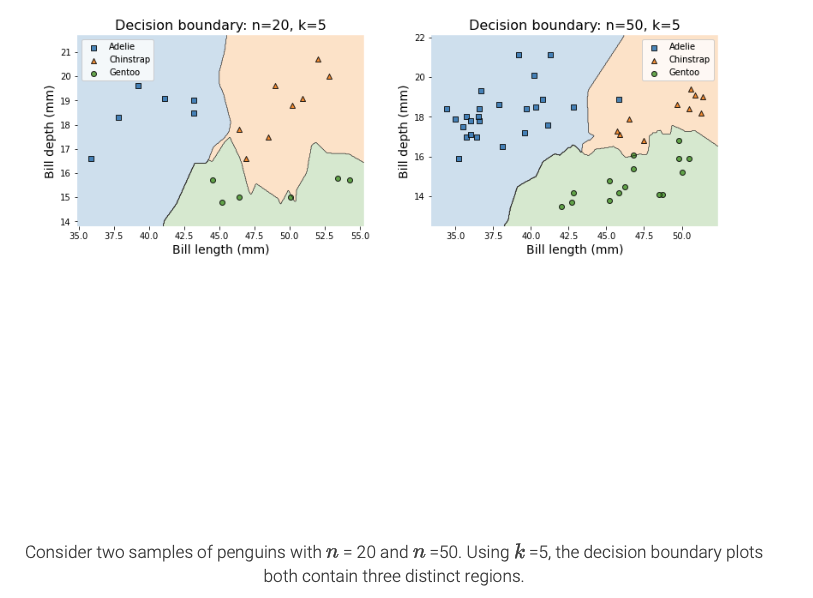
\includegraphics[width=\linewidth]{imgs/knn_29.png}
	\end{figure}
\end{frame}

\begin{frame}
	\frametitle{Exploring classification models with decision boundary plots.}
	\begin{figure}[ht]
		\centering
		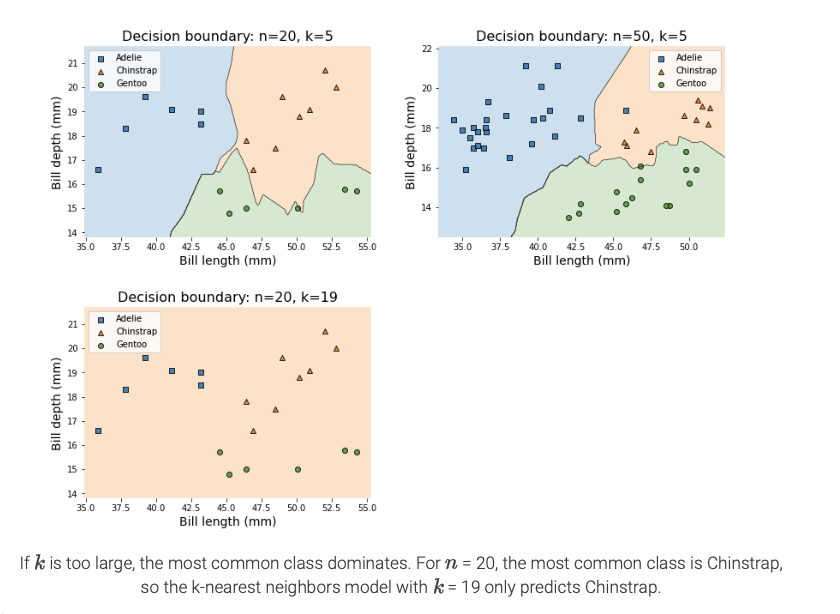
\includegraphics[width=\linewidth]{imgs/knn_30.png}
	\end{figure}
\end{frame}

\begin{frame}
	\frametitle{Exploring classification models with decision boundary plots.}
	\begin{figure}[ht]
		\centering
		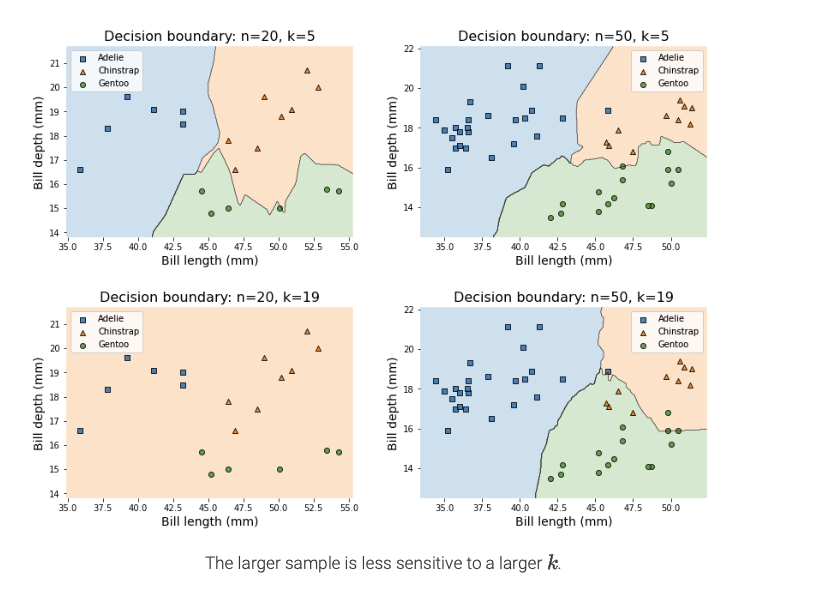
\includegraphics[width=\linewidth]{imgs/knn_31.png}
	\end{figure}
\end{frame}
\begin{frame}{Practice Questions: Effect of k on decision boundaries.}

	\begin{figure}[ht]
		\centering
		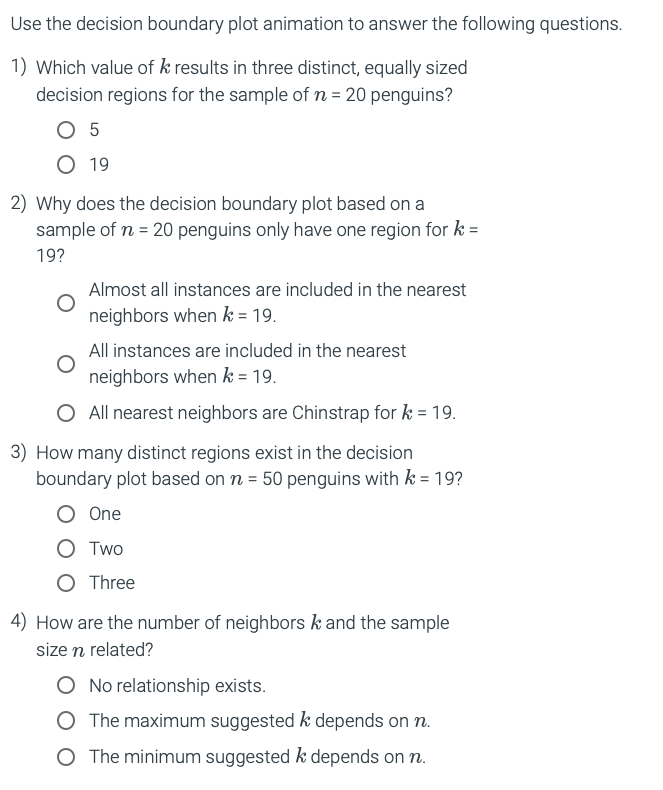
\includegraphics[scale=0.25]{imgs/knn_32.png}
	\end{figure}

\end{frame}

\section{Distance Measures}
\begin{frame}
	\frametitle{Distance Measures}
	k-nearest neighbors classifies instances based on the classes of the \(k\) closest instances.
	\begin{itemize}
		\item But, depending on how the distance between instances is defined, the nearest neighbors may change.
		\item  Three common distance measures for k-nearest neighbors
		      classification are Euclidean distance, Manhattan distance, and Minkowski distance.
	\end{itemize}

\end{frame}
\begin{frame}
	\frametitle{}
	Consider two instances, \(j\) and \(k\), with \(p\) input features.
	\begin{itemize}
		\item  The \textbf{Euclidean distance} between instances \(j\) and \(k\) is
		      $$
			      d_{E}(j, k)=\sqrt{\left(x_{1 j}-x_{1 k}\right)^{2}+\left(x_{2 j}-x_{2 k}\right)^{2}+\ldots\left(x_{p j}-x_{p k}\right)^{2}}=\left(\sum_{i=1}^{p}\left(x_{i j}-x_{i k}\right)^{2}\right)^{1 / 2}
		      $$
		\item \textbf{Manhattan distance}, or city block distance, is based on the absolute difference of the coordinates.
		      $$
			      d_{M}(j, k)=\sum_{i=1}^{p}\left|x_{i j}-x_{i k}\right|
		      $$
		\item \textbf{Minkowski distance}  is a generalized distance measure, with the power allowed to vary.
		      $$
			      d_{m}(j, k)=\left(\sum_{i=1}^{p}\left|x_{i j}-x_{i k}\right|^{1 / m}\right)^{1 / m}
		      $$

		      Euclidean distance is equivalent to Minkowski distance with \(m=2\), and Manhattan distance is equivalent to Minkowski
		      distance with \(m=1\). Different situations may call for different distance measures.
	\end{itemize}
\end{frame}

\begin{frame}
	\frametitle{Calculating distance measures.}
	\begin{figure}[ht]
		\centering
		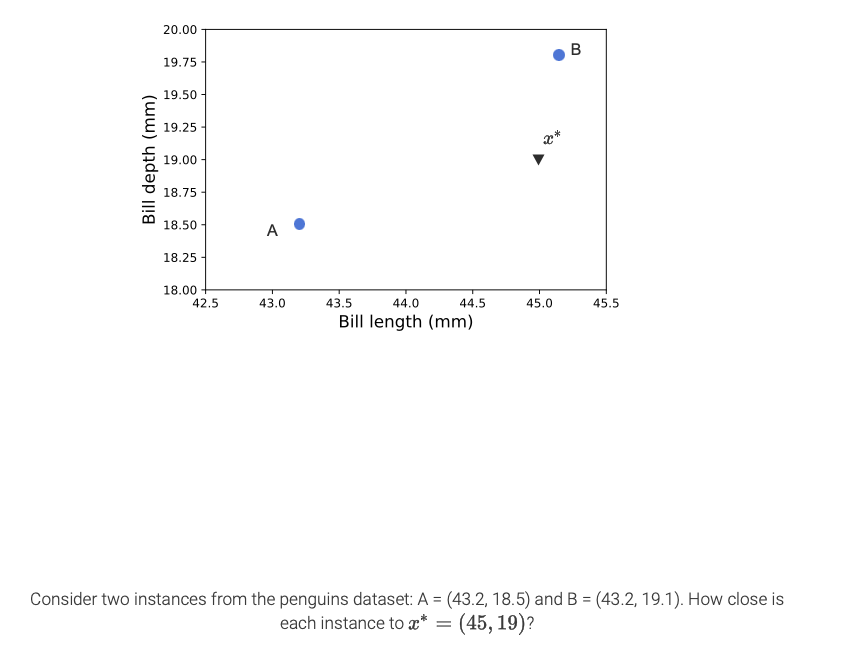
\includegraphics[width=0.7\linewidth]{imgs/knn_33.png}
	\end{figure}
\end{frame}

\begin{frame}
	\frametitle{Calculating distance measures.}
	\begin{figure}[ht]
		\centering
		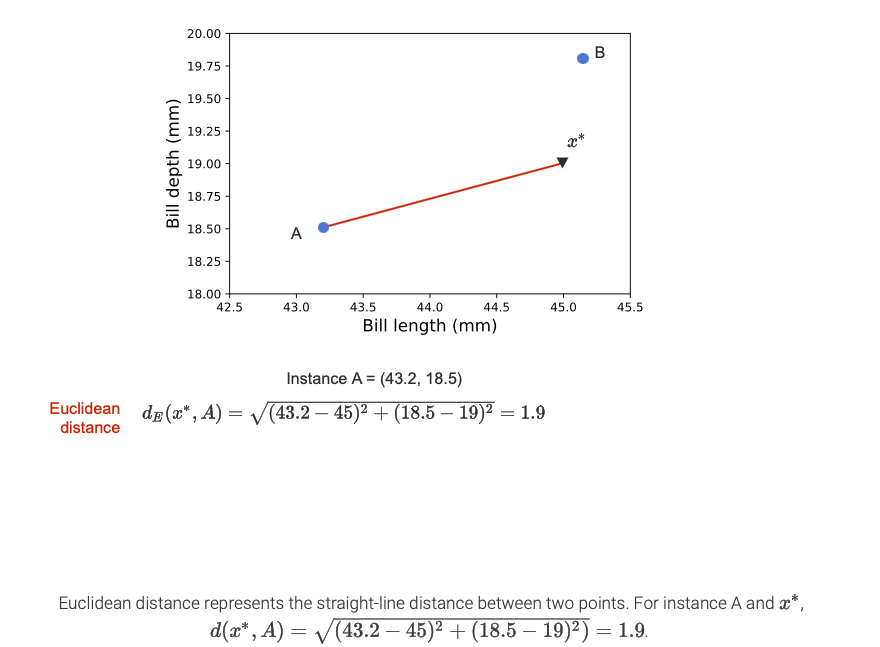
\includegraphics[width=0.7\linewidth]{imgs/knn_34.png}
	\end{figure}
\end{frame}

\begin{frame}
	\frametitle{Calculating distance measures.}
	\begin{figure}[ht]
		\centering
		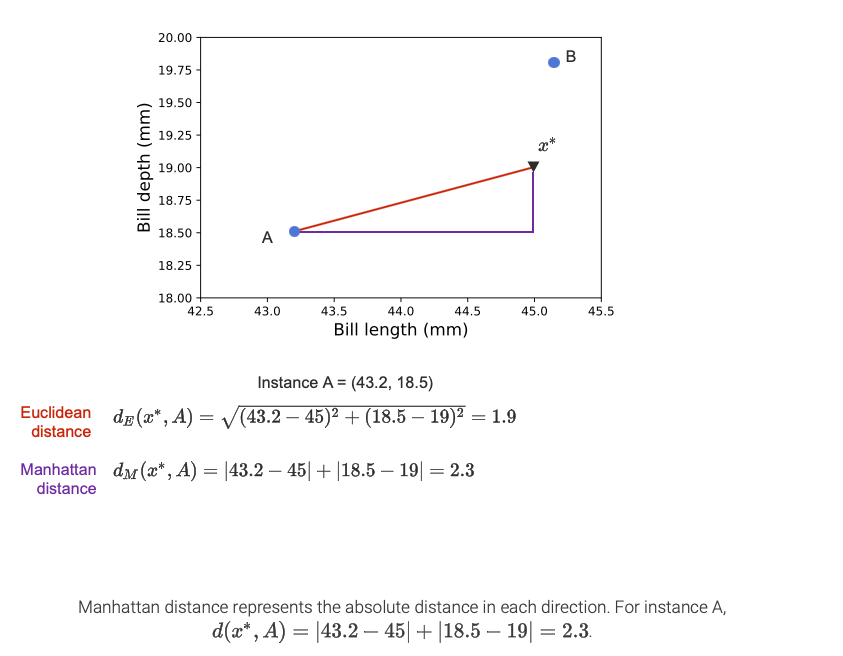
\includegraphics[width=0.7\linewidth]{imgs/knn_35.png}
	\end{figure}
\end{frame}
\begin{frame}
	\frametitle{Calculating distance measures.}
	\begin{figure}[ht]
		\centering
		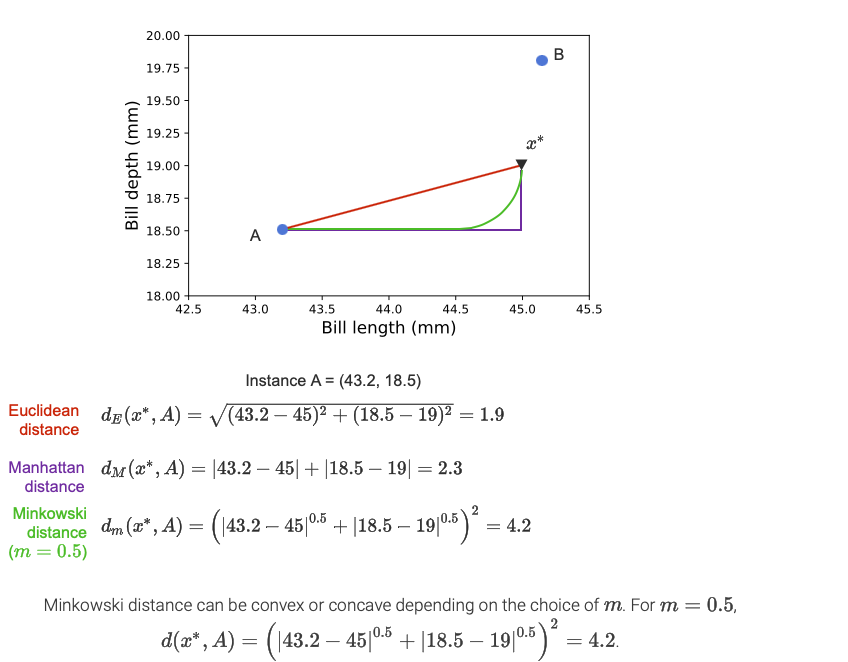
\includegraphics[width=0.7\linewidth]{imgs/knn_36.png}
	\end{figure}
\end{frame}
\begin{frame}
	\frametitle{Calculating distance measures.}
	\begin{figure}[ht]
		\centering
		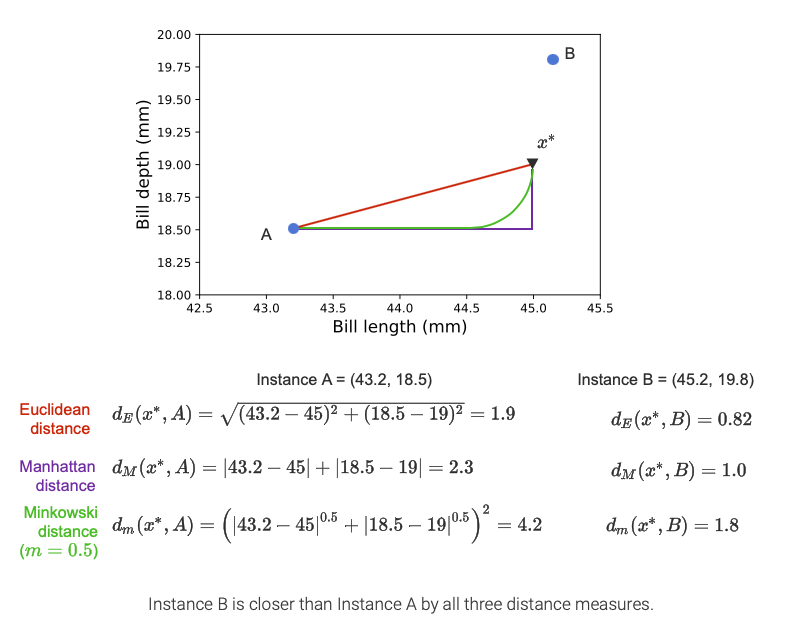
\includegraphics[width=0.7\linewidth]{imgs/knn_37.png}
	\end{figure}
\end{frame}
\section{Advantages and Disadvantages}
\begin{frame}
	\frametitle{Advantages and Disadvantages}
	k-nearest neighbors is a flexible classification model that can predict to any number of classes, but limitations exist.
	\begin{itemize}
		\item 	\textbf{Distance-based algorithms} make predictions based only on the most similar instances, and do not consider relationships between input and output features.
	\end{itemize}
	Since k-nearest neighbors only uses the input features to identify the nearest instances, k-nearest neighbors should not be used to
	describe relationships between input and output features.
\end{frame}

\begin{frame}
	\frametitle{}

	Distance-based algorithms like k-nearest neighbors are sensitive to the unit and magnitude of measurement for each feature.
	\begin{itemize}
		\item Ex: The distance value between the body mass of two penguins depends on whether body mass is measured in grams or kilograms.
		\item Input features in distance-based algorithms should be standardized before fitting a model. Standardized features are scaled to have a mean of 0 and a standard deviation of 1. A feature is standardized by subtracting the mean, \(\bar{x}\), and dividing by the standard deviation, \(s\).
		      $$
			      z=\frac{x-\bar{x}}{s}
		      $$
		      Standardized values are also referred to as z-scores.
	\end{itemize}

\end{frame}
\end{document}